\section*{\centering ABSTRACT}

We present a new approach for generating bas-reliefs from brush paintings. Our approach exploits the concept of brush strokes, making strokes possible to generate correspond bas-relief proxies suitable for recomposing in art design. To segment brush strokes in 2D paintings, we reformulate layer decomposition and MSERs segmentation by imposing boundary constraints, which can make strokes smooth and complete. The resulting 3D proxies of brush strokes are sufficient to evoke the impression of the consistent 3D shapes, so that they may be further edited in 3D space. This fulfills the request of recomposition in bas-relief design. We demonstrate our approach on a variety of brush paintings, showing that even in different styles of brush paintings, 

Bas-relief is an art form part way between sculpture and painting, in this research , we present a new approach for generating aesthetically pleasing bas-reliefs from brush paintings. We do not aim to recover exact depth values for objects in the paintings, which is a hard computer vision problem, requiring assumptions that are rarely satisfied. Instead, our approach exploits the concept of brush strokes, making strokes possible to generate 3D bas relief proxies separately suitable for recomposing in art design. Different paintings have different stroke patterns. Understanding the rules will improve the success rate of a wider range of paintings.Currently, our research focus on brush paintings with relatively sparse and clear strokes. 

As showed in Figure \ref{pip}, the approach performs in three steps: First,  based on the point cloud of the input image in RGB space, we select the palette colors of the input brush painting, and based on the palette colors we decompose a input image into different layers with transparency,  Second,  the original painting is decomposed into element brush strokes by applying modified MSERs segmentation.Based on our observation, alpha map is more suitable for our MSERs segmentation, so the segmentation is based on the transparency. Third, based on the segmented brush strokes,  Shape from Shading algorithm has been applied to generate the depth map of each stroke.  finally, based on those 3D strokes , we can edit the generated bas relief. For editing,we have already generated the 3D proxies for each MSER region, namely, the extracted 2D brush region, so, we can change the depth of specific stroke on bas relief,we can also stitch them on each other based on the user input and change the shape of a certain stroke with given indicated skeleton. By doing so, we fulfill the request of recomposition in bas-relief design.The resulting 3D proxies of brush strokes are sufficient to evoke the impression of the consistent 3D shapes,so that they may be further edited in 3D space. 
Currently, our research focus on brush paintings with relatively sparse strokes.
Experiments show that our method can effectively generate digital bas-reliefs for a range of input images, including some Chinese paintings and rose-mailing paintings.
We also demonstrate the utility of the resulting decompositions for image recoloring and image object insertion and animation.

\begin{figure}[H]
\centering
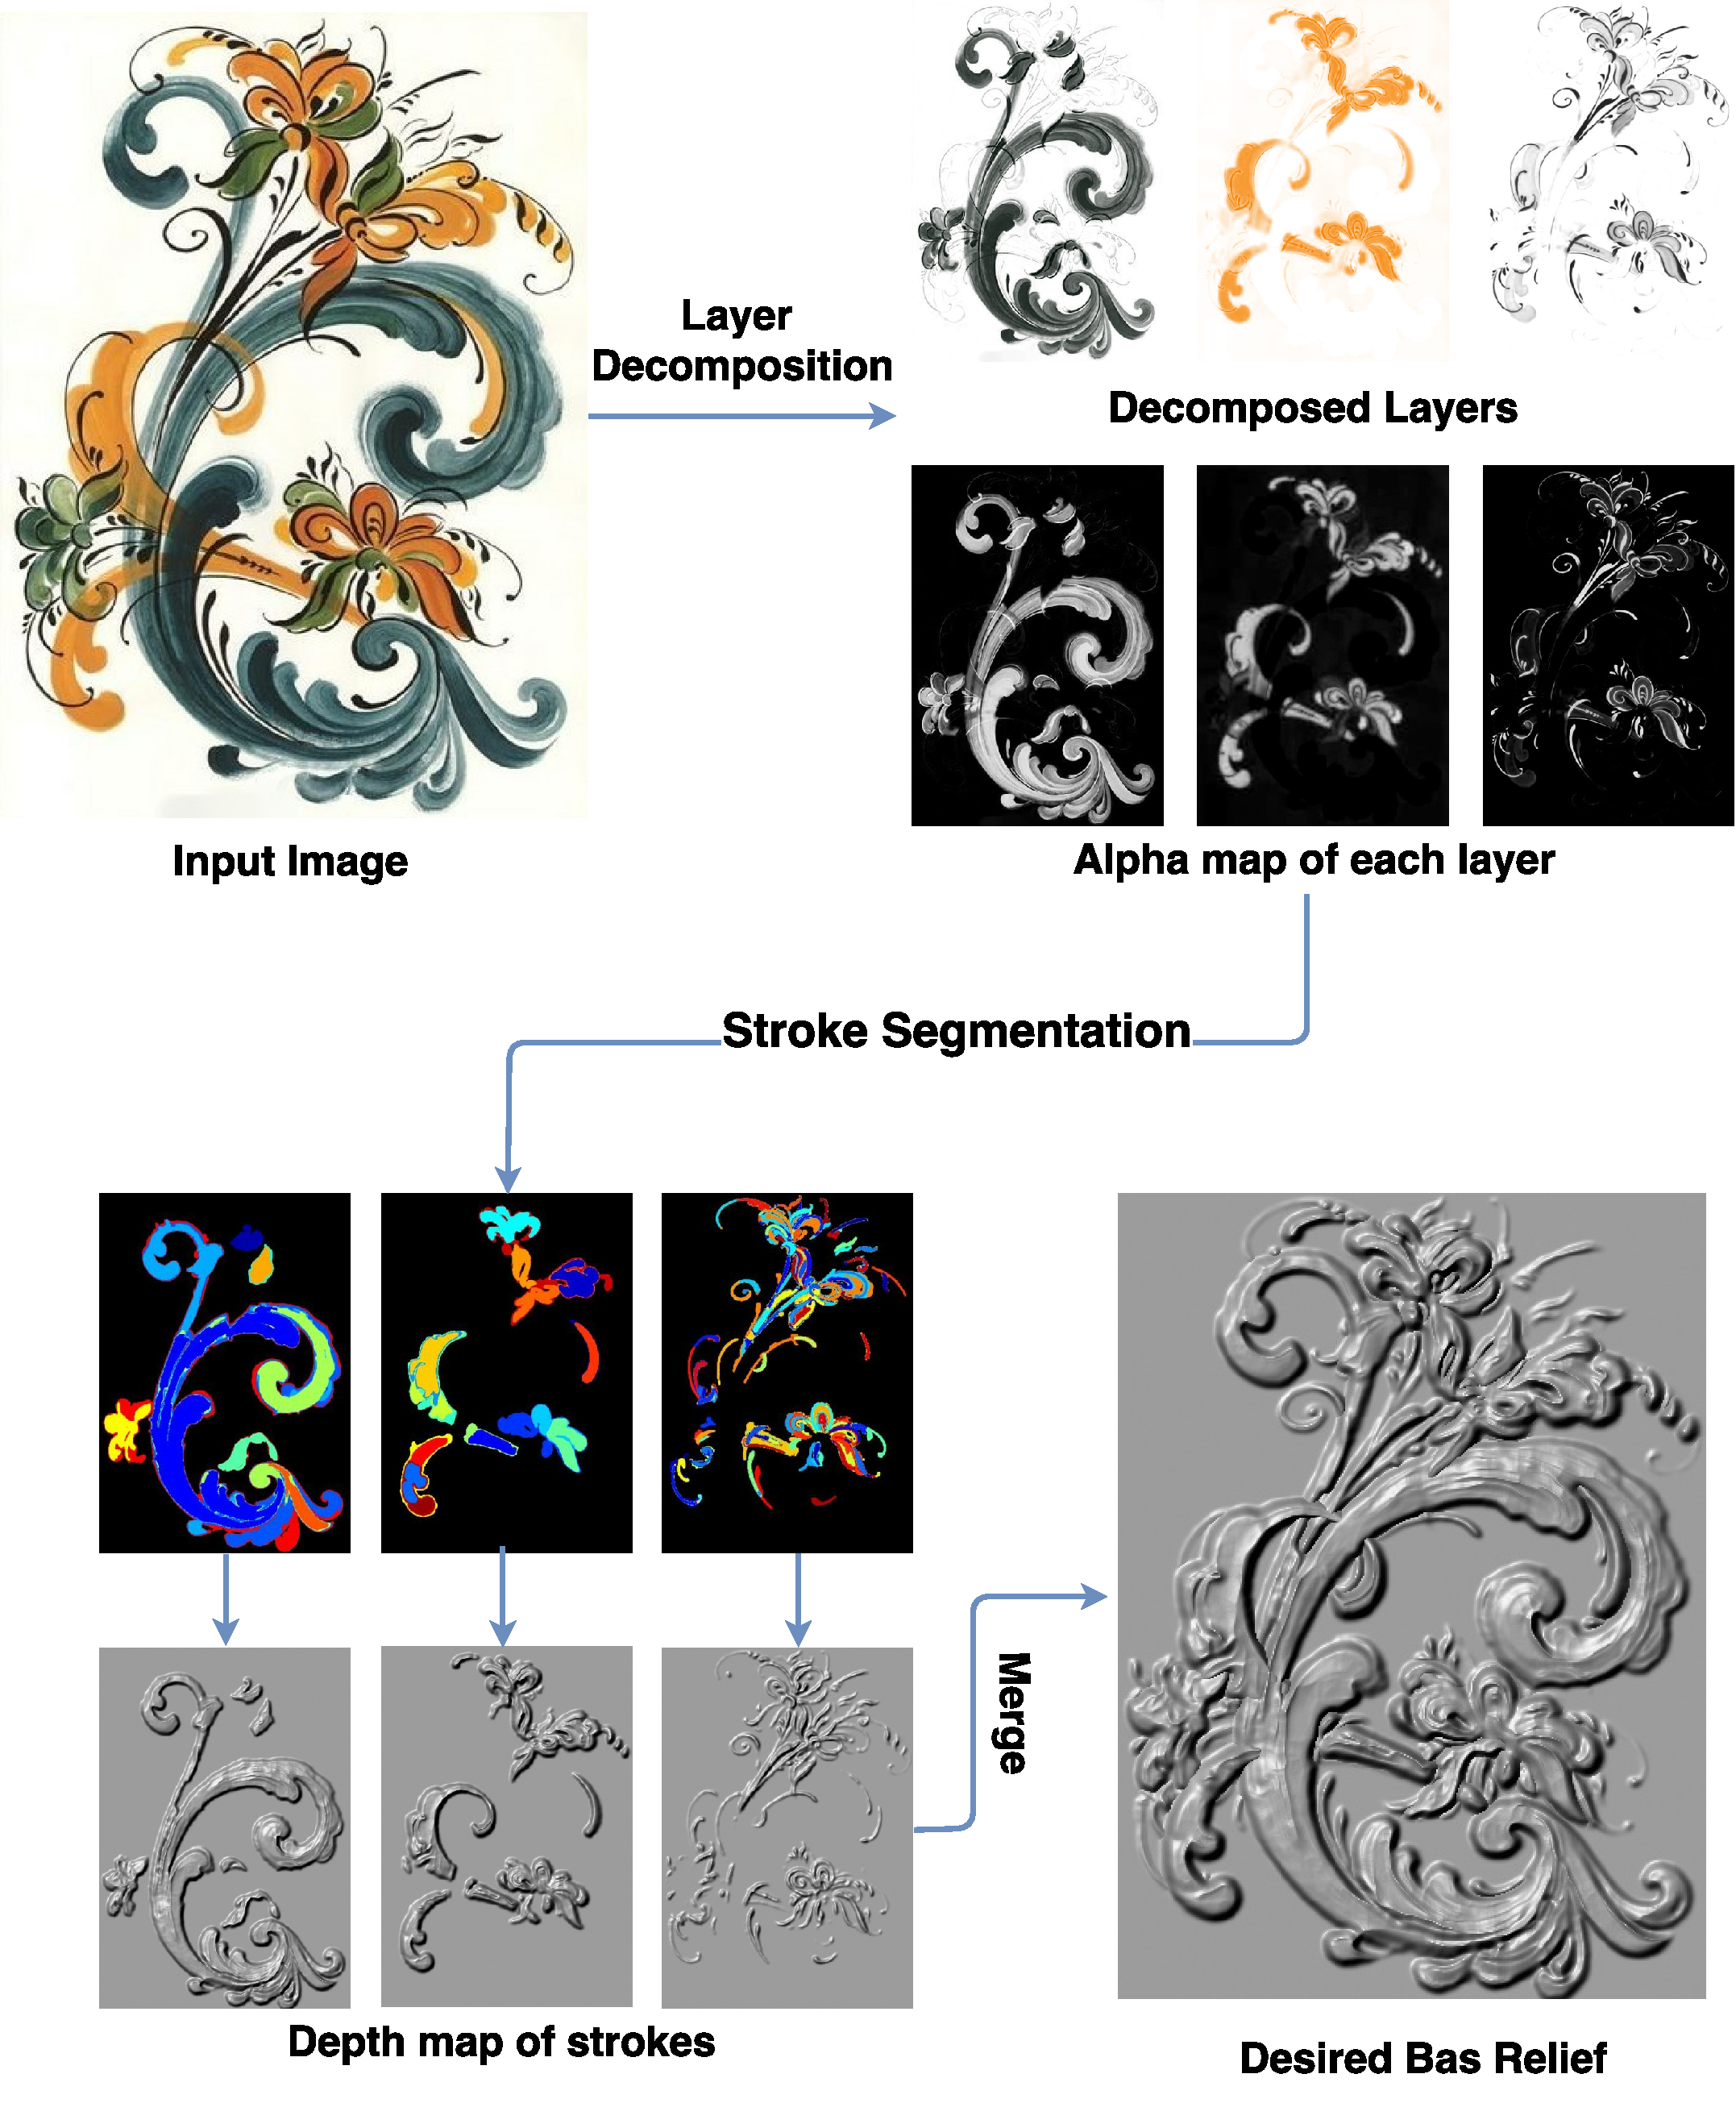
\includegraphics[scale=0.4]{overview.pdf}
\caption{Pipeline Overview}
\label{pip}
\end{figure} 
 
\newpage


 

